% !TeX spellcheck = en_US
%% 
%% Copyright 2007, 2008, 2009 Elsevier Ltd
%% 
%% This file is part of the 'Elsarticle Bundle'.
%% ---------------------------------------------
%% 
%% It may be distributed under the conditions of the LaTeX Project Public
%% License, either version 1.2 of this license or (at your option) any
%% later version.  The latest version of this license is in
%%    http://www.latex-project.org/lppl.txt
%% and version 1.2 or later is part of all distributions of LaTeX
%% version 1999/12/01 or later.
%% 
%% The list of all files belonging to the 'Elsarticle Bundle' is
%% given in the file `manifest.txt'.
%% 

%% Template article for Elsevier's document class `elsarticle'
%% with numbered style bibliographic references
%% SP 2008/03/01

%\documentclass[preprint,12pt]{elsarticle}
%% for a journal layout:
%% \documentclass[final,1p,times]{elsarticle}
%% \documentclass[final,1p,times,twocolumn]{elsarticle}
%% \documentclass[final,3p,times]{elsarticle}
%% \documentclass[final,3p,times,twocolumn]{elsarticle}
%% \documentclass[final,5p,times]{elsarticle}
 \documentclass[final,5p,times,twocolumn]{elsarticle}


\usepackage{amsmath}
\usepackage{graphicx}
\usepackage{float}
\usepackage{amssymb}
\usepackage{caption}
\usepackage{subcaption}

%\usepackage[]{tocbibind} 
%\renewcommand\bibname{References}

% ---------------------------
\graphicspath{{fig/}}
% ---------------------------

%% Use the option review to obtain double line spacing
%% \documentclass[authoryear,preprint,review,12pt]{elsarticle}

%% Use the options 1p,twocolumn; 3p; 3p,twocolumn; 5p; or 5p,twocolumn
%% for a journal layout:
%% \documentclass[final,1p,times]{elsarticle}
%% \documentclass[final,1p,times,twocolumn]{elsarticle}
%% \documentclass[final,3p,times]{elsarticle}
%% \documentclass[final,3p,times,twocolumn]{elsarticle}
%% \documentclass[final,5p,times]{elsarticle}
%% \documentclass[final,5p,times,twocolumn]{elsarticle}

%% For including figures, graphicx.sty has been loaded in
%% elsarticle.cls. If you prefer to use the old commands
%% please give \usepackage{epsfig}

%% The amssymb package provides various useful mathematical symbols
\usepackage{amssymb}
%% The amsthm package provides extended theorem environments
%% \usepackage{amsthm}

%% The lineno packages adds line numbers. Start line numbering with
%% \begin{linenumbers}, end it with \end{linenumbers}. Or switch it on
%% for the whole article with \linenumbers.
%% \usepackage{lineno}

\journal{Progress in Aerospace Sciences}

\begin{document}

\begin{frontmatter}

%% Title, authors and addresses

%% use the tnoteref command within \title for footnotes;
%% use the tnotetext command for theassociated footnote;
%% use the fnref command within \author or \address for footnotes;
%% use the fntext command for theassociated footnote;
%% use the corref command within \author for corresponding author footnotes;
%% use the cortext command for theassociated footnote;
%% use the ead command for the email address,
%% and the form \ead[url] for the home page:
%% \title{Title\tnoteref{label1}}
%% \tnotetext[label1]{}
%% \author{Name\corref{cor1}\fnref{label2}}
%% \ead{email address}
%% \ead[url]{home page}
%% \fntext[label2]{}
%% \cortext[cor1]{}
%% \address{Address\fnref{label3}}
%% \fntext[label3]{}

\title{Voronoi Diagrams Bordering the Escape Regions \\ for the Target-Attacker-Defender Problem}

%% use optional labels to link authors explicitly to addresses:
%% \author[label1,label2]{}
%% \address[label1]{}
%% \address[label2]{}

\author{Mostafa Ali Rushdi, Ayman H. Kassem, Gamal El-Bayoumi} 
\address{Department of Aerospace Engineering\\
Cairo University\\
Cairo, Egypt\\
\tt morushdi@gmail.com, draymank@yahoo.com, gelbayoumi@yahoo.com}

%% ===================================================
\begin{abstract}
This paper deals with an important pursuit-evasion problem that involves three agents, the Target the Attacker and the Defender. The Attacker missile pursues a Target aircraft that is being helped by a Defender missile which tries to intercept the Attacker before it reaches the Target. A differential game arises in which a team is formed by the Target and the Defender which cooperate to maximize the separation between the Target and the point where the Defender intercepts the Attacker, while the Attacker tries to minimize this separation. This paper offers a unified analytic treatment of the aforementioned problem based on the construction of two Apollonius circles. The treatment includes all possibilities of the ratio between the speeds of the Attacker and Defender. A criticality condition is derived from which two important entities are obtained, namely: (a) the critical Target speed normalized wrt the Attacker's speed, and (b) the Voronoi diagram bordering the safe or escape region for the Target. Beside unifying previously published results in a common setting, this paper simplifies all computations by using intuitionistic plane-geometric arguments rather than the more tedious analytic-geometric manipulations. Moreover, the paper extends existing results by adding some novel results, thereby giving a complete picture of all cases of interest. The analysis in this paper is supplemented by extensive computations using MATLAB to plot the Voronoi diagrams under a variety of pertinent parameters. The numerical results and plots obtained allow useful and insightful interpretation.

\end{abstract}

\begin{keyword}
Pursuit-Evasion, Target, Attacker, Defender, Apollonius circle, critical speed ratio, Escape region, Voronoi diagram.
\end{keyword}

\end{frontmatter}

%% \linenumbers
%% ===================================================
\section{Introduction}
\noindent This paper deals with a scenario of active target defence involving three-agent pursuit-evasion where each agent has a specific role. A two-agent team consists of a Target (aircraft) and a Defender (missile) cooperating in opposition to an Attacker (missile). The Target tries to evade the Attacker and avoid being captured by him. The Defender cooperates with and assists the Target by trying to intercept(capture and destroy) the Attacker before the latter captures the Target \cite{pachter2014active,garcia2015active,garcia2015escape,garcia2014cooperative,garcia2015cooperative,garcia2015cooperative2}.
This problem will be referred to herein as the $TAD$ problem as it concerns a triad consisting of the Target($T$), Attacker($A$), and Defender($D$).

The $TAD$ problem constitutes a dynamic differential game \cite{ho1965differential,isaacs1954differential,meier1969new,hsueh2007differential,yi2010improved,bressan2010noncooperative,perelman2011cooperative,battistini2014differential,yavin2014pursuit} and is of interest in aerospace, control, and robotics engineering. We will consider herein recent formulation and treatments of this problem \cite{pachter2014active,garcia2015active,garcia2015escape,garcia2014cooperative,garcia2015cooperative,garcia2015cooperative2}, though there exist other formulations and treatments of it that span almost half a century \cite{boyell1976defending,shneydor1977comments,rusnak2005lady,rusnak2008guidance,de2010analysis,rusnak2011guidance,fuch2011encouraging,scott2013pursuit,rubinsky2013three,oyler2014pursuit}.
Table \ref{tableTAD} shows several variants of this generic problem in a variety of settings, contexts or disciplines. The $TAD$ problem is a generalization of the classical problem of a single pursuer and a single evader \cite{anderson1978model,miller1994co,cliff1995co,pekalski2004short,zarchan2002tactical}. In fact, the $TAD$ is essentially a duplication of this classical problem, since in the $TAD$ problem, the Attacker plays the double role of being a pursuer for the Target, and at the same time an evader for the Defender \cite{rusnak2008guidance}.
The $TAD$ problem is also a special case of a more general pursuit-evasion problem in which there are multiple Attackers and multiple Defenders  \cite{hagedorn1976differential,kim2001multiagent,fuchs2010cooperative,pan2012pursuit,ragesh2014analysis}. Many common threads are shared by all these problems, such as the solution of differential games \cite{ho1965differential,isaacs1954differential,meier1969new,hsueh2007differential,yi2010improved,bressan2010noncooperative,perelman2011cooperative,battistini2014differential,yavin2014pursuit} and the construction of Apollonius circles \cite{ayoub2003proving,ayoub2006circle,partensky2008circle,fulton2015conflict} and Voroni diagrams \cite{gowda1983dynamic,aurenhammer1991voronoi,cheung2007pursuit,gavrilova2008generalized,majdandzic2008computation,bakolas2010optimal,bakolas2010zermelo,bakolas2010optimal}.

\begin{table*}[htb]
  \centering
  \caption{A variety of settings or contexts for the same generic problem}
\begin{tabular}{ |c||c|c|c|c| } 
\hline
Area & Agent 1 & Agent 2 & Agent 3 & References \\
 \hline
 \hline
 Aerospace & Target & Attacker(missile) & Defender(missiles) & \cite{pachter2014active,garcia2015active,garcia2015escape,garcia2014cooperative,garcia2015cooperative}\\
 \hline 
 Biology & Prey & Predator & Protector & \cite{de2010analysis,oyler2014pursuit}\\
 \hline 
 Society & Lady & Bandits & Bodyguards & \cite{rusnak2005lady}\\ 
 \hline
 Criminology & Robber & Policemen/Cops & Gangsters & \cite{cheung2007pursuit}\\ 
  \hline
\end{tabular}
%\caption{A variety of settings or contexts for the same generic problem}
\label{tableTAD}
\end{table*}  

This paper offers a unified analytic treatment of the aforementioned $TAD$ problem based on the construction of two Apollonius circles.
The treatment includes all possibilities of the ratio between the speeds of the Attacker and Defender.Note that the case of a slow Defender appears here for the first time, while the treatment of the cases of fast Defender or similar Defender is extended and augmented with novel results and new insights. A criticality condition is derived from which the two following important entities are obtained
\begin{itemize}
\item the critical Target speed normalized w.r.t. the Attacker's speed so as to be a dimensionless quantity,
\item the Voronoi diagram bordering the safe or escape region for the Target.
\end{itemize}

Beside unifying previously published results in a common setting, this paper simplifies all computations by using intuitionistic plane-geometric arguments rather than the more tedious analytic-geometric manipulations. 
Moreover, the paper extends existing results by adding some novel results, thereby giving a complete picture of all cases of interest.
The analysis in this paper is supplemented by extensive computations using MATLAB to solve the complex high-order polynomial equations and to plot the Voronoi diagrams under a variety of pertinent parameters. The numerical results and plots obtained allow useful and insightful interpretations.
\\
\\
The organization of the remainder of this paper is as follows. Section II lists the assumptions, notation and nomenclature used herein. Section III discusses the general concepts and properties of an Apollonius circle \cite{ayoub2003proving,ayoub2006circle,partensky2008circle,fulton2015conflict}, and then specializes these to the cases of the $AD$ Apollonius circle and the $TA$ Apollonius circle. Section IV derives a criticality condition which constitutes a quadratic equation that is later solved for the critical dimensionless ratio between the Target speed and Attacker speed. The same criticality condition is then rephrased in Section V as a relation between the initial coordinates $x_T$ and $y_T$ of the Target. This relation leads to the Voronoi diagram bordering the \textit{safe} or \textit{escape} region $R_e$ of the Target. This Voronoi diagram is published for the first time when the Defender is fast or slow. It includes as a special case the much simpler diagram for a similar Defender that has already appeared in \cite{garcia2015escape}. Section VI concludes the paper and points out possible directions for further work.  

% =========================================

\section{ASSUMPTIONS, NOTATION, AND NOMENCLATURE}

\subsection{ASSUMPTIONS}
\begin{enumerate}
\item The speeds $V_{T},V_{A},$ and $V_{D}$ of the Target, Attacker, and Defender are constant.
\item The Attacker missile is faster than the Target aircraft, i.e., $\alpha\equiv \dfrac{V_{T}}{V_{A}}<1$ (In the case $\alpha\geq1$, the Target is guaranteed to survive by following an optimal strategy, even without assistance from the Defender).
\item There are three distinct cases for the ratio of the speed of the Attacker to that of the Defender $\gamma=\dfrac{1}{\beta}=\dfrac{V_{A}}{V_{D}}$ 
\begin{itemize}
\item $\gamma<1$ (fast Defender) discussed earlier in Garcia et el. \cite{garcia2015active}, and extended, expounded, simplified and exposed herein.
\item $\gamma =1$ (same speed Defender) discussed in Garcia et el. \cite{pachter2014active,garcia2015escape}, and extended, expounded, simplified and exposed herein.
\item $\gamma>1$ (slow Defender), which is a novel case, discussed herein for the first time, and unified with the two previous cases.  
\end{itemize}

\item The Defender intercepts the Attacker if their separation becomes zero (point capture).
\item The optimal trajectories of the three agents are straight lines.
\item A Cartesian frame is attached to the initial positions $A$ and $D$ of the Attacker and Defender in such a way the $X$-axis is the infinite extension of the straight segment $\overline{AD}$ and the $Y$-axis is the perpendicular bisector of $\overline{AD}$.
\end{enumerate}

\subsection{NOTATION}
\begin{itemize}
\item $A$: Initial position of the Attacker.
\item $D$: Initial position of the Defender.
\item $T$: Initial position of the Target.
\item $T'$ Terminal position of the Target, i.e., its position at the time the Defender intercepts the Attacker.
\item $\alpha=\dfrac{V_{T}}{V_{A}}$ (assumed $<1$, otherwise the target trivially survives).
\item $\gamma=\dfrac{1}{\beta}=\dfrac{V_{A}}{V_{D}}$ (studied for a fast Defender ($\gamma<1$), a similar Defender ($\gamma=1$), and a slow Defender ($\gamma>1$)).
\item $u, v, w$: Aim points on the $AD$ Apollonius circle by the Attacker, Target and Defender, respectively. 
\end{itemize}

\subsection{NOMENCLATURE}
\subsubsection{The $AD$ Apollonius circle}
The locus of a point such that the ratio of its distance from the initial positions $\boldsymbol{A}=(x_{A},0)$ and $\boldsymbol{D}=(-x_{A},0)$ of the Attacker and Defender, respectively, is a fixed ratio $\gamma=\dfrac{V_{A}}{V_{D}}$. This circle degenerates into the perpendicular bisector of $\overline{AD}$ if $\gamma=1$.
Points on the circumference of this circle are reached simultaneously by the Attacker and Defender. For $\gamma<1$, $\boldsymbol{A}$ belongs to the interior of this circle and points within the circle are reached by the Attacker before the Defender. For $\gamma>1$, $\boldsymbol{D}$ belongs to the interior of this circle and points within the circle are reached by the Defender before the Attacker. For $\gamma=1$, the $AD$ circle becomes of infinite radius and degenerates into a straight line, namely the perpendicular bisector of $\overline{AD}$. In this case, $\boldsymbol{A}$ belongs to the R.H.S. of the $XY-$plane where points are reached by the Attacker before the Defender, while $\boldsymbol{D}$ belongs to the L.H.S. of the $XY-$plane where points are reached by the Defender before the Attacker.   

\subsubsection{The $TA$ Apollonius circle} 
The locus of a point such that the ratio of its distances from the initial positions $\boldsymbol{T}=(x_{T},y_{T})$ and $\boldsymbol{A}=(x_{A},0)$, of the Target and Attacker, respectively, is a fixed ratio $\alpha= \dfrac{V_{T}}{V_{A}}$ strictly less than 1. Naming of the $AD$ and $TA$ Apollonius circles herein follows a common practice in mathematical circles \cite{ayoub2003proving,ayoub2006circle,partensky2008circle} and is opposite to the style used by Garcia et al. \cite{pachter2014active,garcia2015active,garcia2015escape}.

\subsubsection{Region reachable by the Defender before the Attacker (Reachability region $R_r$)}
For $\gamma<1$, $R_r$ is the exterior of the $AD$ Apollonius circle.\\
For $\gamma=1$, $R_r$ is the L.H.S. of the $XY-$plane.\\
For $\gamma>1$, $R_r$ is the interior of the $AD$ Apollonius circle. 

Figure \ref{Rr2} illustrates this region as a shaded region to which point $D$ belongs.

\begin{figure*}
\centering
\begin{subfigure}[htb]{0.3\textwidth}
\includegraphics[width=\columnwidth]{drawing4_1a.pdf}
\caption {$\gamma<1$}
\label{2_g<1}
\end{subfigure}
\quad
\begin{subfigure}[htb]{0.3\textwidth}
\includegraphics[width=\columnwidth]{drawing4_1b.pdf}
\caption {$\gamma=1$}
\label{2_g=1}
\end{subfigure}
\quad
\begin{subfigure}[htb]{0.3\textwidth}
\includegraphics[width=\columnwidth]{drawing4_1c.pdf}
\caption {$\gamma>1$}
\label{2_g>1}
\end{subfigure}
\caption{The reachability region $R_r$ (one including $\boldsymbol{D}$ whose points are reached by the Defender before the Attacker) is shown shaded.}
\label{Rr2}
\end{figure*}

\subsubsection{Region of guaranteed Target's escape (Escape region $R_e$)}
The escape region $R_e$ is the set of all coordinate pairs $(x,y)$ such that if the Target initial position $\boldsymbol{T}=(x_{T},y_{T})$ is inside this region, then it is guaranteed to escape the Attacker if both the Target and Defender implement their corresponding optimal strategies. This set is a strict superset of the set of points reachable by the Defender before the Attacker ($R_e\supseteq R_r$). The boundary of this set is called a Voronoi Diagram.

\subsubsection{The critical speed ratio $\overline{\alpha}$}
A lower limit on the speed ratio $\gamma=\dfrac{V_{T}}{V_{A}}$, attained when the $TA$ Apollonius circle is tangent to the $AD$ Apollonius circle (or to the perpendicular bisector of $\overline{AD}$ in the degenerate case $\gamma=1$).   

\subsubsection{Escape Condition}
For a given speed ratio $\alpha=\dfrac{V_{T}}{V_{A}}$ and a given Attacker's initial position $\boldsymbol{A}=(x_{A},0)$, the escape condition is that the $TA$ Apollonius circle (of center $O_2$ and radius $r_2$) intersects the $AD$ Apollonius circle (of center $O_1$ and radius $r_1$). This happens for $\gamma<1$ when
\begin{equation}
\lvert \boldsymbol{O_{1}}-\boldsymbol{O_{2}}\rvert+r_{2}>r_{1}
\end{equation}
It happens for $\gamma>1$ when
\begin{equation}
\lvert \boldsymbol{O_{1}}-\boldsymbol{O_{2}}\rvert-r_{2}<r_{1}
\end{equation}
In the degenerate case of $\gamma=1$, it is required that the $TA$ Apollonius circle intersects the $Y-$axis, i.e., 
\begin{equation}
r_{2}>the\ abscissa\ of\ \boldsymbol{O_{2}}
\end{equation}


% =========================================

\section{APOLLONIUS CIRCLES PERTAINING TO THE \textit{TAD} PROBLEM}
A circle is the locus moving at a constant distance (called the circle's radius $r$) from a fixed point (called the circle's centre $O$).
In the limit of an infinite radius $(r\longrightarrow\infty∞)$, the circle degenerates into a straight line.
Another definition of the circle is that it is the locus of a point moving such that the ratio of its distances from two fixed points A and B is a constant $k$. With this definition, the circle is called a circle of Apollonius (in honour of Apollonius of Perga (ca. 262-190 BC), the Great Geometer of Antiquity). In the limit ($k\longrightarrow1$) this circle degenerates into the perpendicular bisector of $\overline{AD}$, while in the two limits ($k\longrightarrow0$) and ($k\longrightarrow\infty$), this circle collapses to the two points A and B, respectively. \\

Two Apollonius circles are studied herein, namely the $AD$ Apollonius circle, and the $TA$ Apollonius circle. The study will be based on simple and intuitive plane-geometric arguments and will avoid the more involved treatment of analytic geometry. Figures \ref{1} and \ref{2} shows the Apollonius circles for a moving point $P$ such that $\dfrac{AP}{PB}=k\neq1$. The case $k>1$ is shown in Fig. \ref{1}, while the case $k<1$ is shwon in Fig. \ref{2}. The points $I$ and $E$ are the two special cases of $P$ that lie on the straight line extension of the straight segment $\overline{AB}$. These points divide the straight segment $\overline{AB}$ internally and externally in the ratio $k\ (k\neq1)$, i.e., 

\begin{equation}
  %\tag{*}
  \boxed{
  \dfrac{AI}{IB}=\dfrac{AE}{EB}=k,\ \{k\neq1\}.}
  \label{eqn:kratio}
\end{equation} 


\begin{figure}[htb]
\centering
\includegraphics[width=0.75\columnwidth]{drawing1.pdf}
\caption{Apollonius circle for a moving point $P$ such that $\dfrac{AP}{PB}=k>1$. Here $m\angle API = m\angle BPI$ and $m\angle A'PE = m\angle BPE$.}
\label{1}
\end{figure}

\begin{figure}[htb]
\centering
\includegraphics[width=0.75\columnwidth]{drawing2.pdf}
\caption{Apollonius circle for a moving point $P$ such that $\dfrac{AP}{PB}=k<1$. Here $m\angle API = m\angle BPI$ and $m\angle APE = m\angle B'PE$.}
\label{2}
\end{figure}

If we denote the position vector of a point by a bold version of its name, we can rewrite \eqref{eqn:kratio} in vectorial form as

\begin{equation}
(\boldsymbol{I}-\boldsymbol{A})=k(\boldsymbol{B}-\boldsymbol{I}),
\end{equation}

\begin{equation}
(\boldsymbol {E}-\boldsymbol{A})=k(\boldsymbol{E}-\boldsymbol{B}),
\end{equation}

which can be used to express $\boldsymbol{I}$ and $\boldsymbol{E}$ in terms of $\boldsymbol{A}$ and $\boldsymbol{B}$ as 
\begin{equation}
\boldsymbol{I} = \dfrac{1}{k+1} (\boldsymbol{A}+k\boldsymbol{B}),
\label{eqn:ipoint}
\end{equation}

\begin{equation}
\boldsymbol{E} = \dfrac{1}{k-1} (-\boldsymbol{A}+k\boldsymbol{B}).
\label{eqn:epoint}
\end{equation}

The Apollonius circle is easily characterized by the points $\boldsymbol{I}$ and $\boldsymbol{E}$, since they are the two end points of one of the its diameters. The center of the circle is the midpoint of points $\boldsymbol{I}$ and $\boldsymbol{E}$, namely:

\begin{equation}
\begin{split}
\boldsymbol{O} & = \dfrac{1}{2} (\boldsymbol{I}+\boldsymbol{E})\\
& = \dfrac{1}{2} [(\dfrac{1}{k+1}-\dfrac{1}{k-1})]\boldsymbol{A}+k(\dfrac{1}{k+1}+\dfrac{1}{k-1}) \boldsymbol{B}\\
& =-\dfrac{1}{k^{2}-1}\boldsymbol{A} + \dfrac{{k^{2}}}{k^{2}-1} \boldsymbol{B},
\end{split}
\label{eqn:center}
\end{equation}

while the radius of the circle is half the length of the displacement from $\boldsymbol{I}$ to $\boldsymbol{E}$,
\begin{equation}
\begin{split}
r & =\dfrac{1}{2} \lvert \boldsymbol{I} -\boldsymbol{E}\rvert \\
& = \dfrac{1}{2} \lvert (\dfrac{1}{k+1}+\dfrac{1}{k-1})\boldsymbol{A}+k(\dfrac{1}{k+1}-\dfrac{1}{k-1}) \boldsymbol{B}\rvert \\
& =  \lvert\dfrac{k}{k^{2}-1}\boldsymbol{A} - \dfrac{k}{k^{2}-1} \boldsymbol{B}\rvert\\
& = \lvert\dfrac{k}{k^{2}-1}\rvert \lvert\boldsymbol{A} -\boldsymbol{B}\rvert = \dfrac{k}{k^{2}-1}(AB).
\end{split}
\label{eqn:radius}
\end{equation}

It is clear from \eqref{eqn:center} and \eqref{eqn:radius} that $\lim_{k\to1}\lvert\boldsymbol{O}\rvert\to\infty$ and $\lim_{k\to1}r\to\infty$, and hence for $k=1$, the Apollonius circle degenerates into a straight line, namely the perpendicular bisector of the straight segment $\overline{AB}$ (Fig. \ref{3}).

\begin{figure}[htb]
\centering
\includegraphics[width=0.75\columnwidth]{drawing3.pdf}
\caption{For $k=1$, the Apollonius circle in figures \ref{1} or \ref{2} degenerates into the perpendicular bisector of the straight segment $\overline{AB}$. The point $E$ disappears in this figure as it goes to $\infty$  }
\label{3}
\end{figure}

\subsection{The $AD$ Apollonius circle}
For the $AD$ Apollonius circle, the two fixed points are the initial positions of the Attacker $\boldsymbol{A}=(x_{A},0)$ and the initial position of the defender $\boldsymbol{D}=(-x_{A},0)$. The fixed ratio of the circle $k$ is replaced by the following dimensionless ratio which is the Attacker's speed normalized w.r.t the Defender speed: 
\begin{equation}
\gamma = \dfrac{V_{A}}{V_{D}}.
\end{equation}
We will consider the three cases of 

\begin{enumerate}
\item $\gamma<1$ (fast Defender) discussed in Garcia et al. \cite{garcia2015active}.
\item $\gamma =1$ (same-speed Defender) discussed in Garcia et al. \cite{pachter2014active, garcia2015escape}.
\item $\gamma>1$ (slow Defender), which is a novel case. 
\end{enumerate}

Substituting the values of $\boldsymbol{A}$ and $\boldsymbol{D}$ above for $\boldsymbol{A}$ and $\boldsymbol{B}$ in \eqref{eqn:ipoint},\eqref{eqn:epoint},\eqref{eqn:center} and \eqref{eqn:radius}, respectively, and replacing $k$ therein by $\gamma$ we obtain for $\gamma\neq1$,

\begin{eqnarray}
\boldsymbol{I_{1}} &=& (\dfrac{1-\gamma}{1+\gamma}x_{A},0),\\
\boldsymbol{E_{1}} &=& (\dfrac{1+\gamma}{1-\gamma}x_{A},0),\\
\boldsymbol{O_{1}} &=& (\dfrac{1+\gamma^{2}}{1-\gamma^{2}}x_{A},0),\\
\label{O1}
r_{1} &=& \dfrac{2\gamma}{\lvert1-\gamma^{2}\rvert}x_{A}.
\label{r1}
\end{eqnarray}

Three interesting sets of limits are now considered. The first set of limits are those when ($\gamma\to1$), namely 

\begin{eqnarray}
\lim_{\gamma\to1} \boldsymbol{I}_1 &=& (0,0),\\
\lim_{\gamma\to1} \boldsymbol{E}_1 &=& (\mp\infty,0),\\
\lim_{\gamma\to1} \boldsymbol{O}_1 &=& (\mp\infty,0),\\
\lim_{\gamma\to1} r_1 &=& \infty,
\end{eqnarray}

which means that the $AD$ Apollonius circle degenerates in the limit ($\gamma\to1$) to a circle of an infinite radius with center still on the $x-$axis but infinitely distant from the origin. More precisely, this limit is identified as a straight line, namely the perpendicular bisector of the straight-line segment $\overline{AD}$.

The second set of limits are those when ($\gamma\to0$), namely 

\begin{eqnarray}
\lim_{\gamma\to0} \boldsymbol{I}_1 &=& (x_A,0),\\
\lim_{\gamma\to0} \boldsymbol{E}_1 &=& (x_A,0),\\
\lim_{\gamma\to0} \boldsymbol{O}_1 &=& (x_A,0),\\
\lim_{\gamma\to0} r_1 &=& 0,
\end{eqnarray}

which means that the $AD$ Apollonius circle collapses in the limit ($\gamma\to0$) to a single point, namely the initial position of the Attacker $\boldsymbol{A}=(x_A,0)$.

The third set of limits are those when ($\gamma\to\infty$), namely
\begin{eqnarray}
\lim_{\gamma\to\infty} \boldsymbol{I}_1 &=& (-x_A,0), \\
\lim_{\gamma\to\infty} \boldsymbol{E}_1 &=& (-x_A,0),\\
\lim_{\gamma\to\infty} \boldsymbol{O}_1 &=& (-x_A,0),\\
\lim_{\gamma\to\infty} r_1 &=& 0,
\end{eqnarray}

which means that the $AD$ Apollonius circle collapses in the limit ($\gamma\to\infty$) to a single point, namely the initial position of the Defender $\boldsymbol{D}=(-x_A,0)$.

\subsection{The $TA$ Apollonius circle}
For the $TA$ Apollonius circle, the two fixed points are the initial position of the Target $\boldsymbol{T}=(x_{T},y_{T})$ and the initial position of the Attacker  $\boldsymbol{A}=(x_{A},0)$.
Again, the fixed ratio of the circle $k$ is replaced by a dimensionless quantity, namely the Target's speed normalized w.r.t. the Attacker's speed: 
\begin{equation}
\alpha= \dfrac{V_{T}}{V_{A}}.
\end{equation}

Here, we will consider only the case $\alpha <1$, since for $\alpha\geqslant1$, the Target always survives, even without any assistance from the Defender.

Now, we substitute the values of $\boldsymbol{T}$ and $\boldsymbol{A}$ above for $\boldsymbol{A}$ and $\boldsymbol{B}$ in \eqref{eqn:ipoint},\eqref{eqn:epoint},\eqref{eqn:center} and \eqref{eqn:radius}, respectively, and replace $k$ therein by $\alpha$ to obtain:

\begin{equation}
\boldsymbol{I_{2}} =\dfrac{1}{1+\alpha}(\boldsymbol{T}+\alpha \boldsymbol{A}) =\dfrac{1}{1+\alpha}(x_{T}+\alpha x_{A},y_{T}),
\end{equation}

\begin{equation}
\boldsymbol{E_{2}} =\dfrac{1}{\alpha-1}(-\boldsymbol{T}+\alpha \boldsymbol{A}) =\dfrac{1}{1-\alpha}(x_{T}-\alpha x_{A},y_{T}),
\end{equation}

\begin{equation}
\boldsymbol{O_{2}} =\dfrac{1}{1-\alpha^{2}}(\boldsymbol{T}-\alpha^{2} \boldsymbol{A}) =\dfrac{1}{1-\alpha^{2}}(x_{T}-\alpha^{2} x_{A},y_{T}),
\label{O2}
\end{equation}

\begin{equation}
r_{2} =\dfrac{\alpha}{1-\alpha^{2}}(TA)
 = \dfrac{\alpha d}{1-\alpha^{2}},
 \label{r2}
\end{equation}

where $d=TA=$ the initial distance between the target and Attacker, namely
\begin{equation}
d=\sqrt{(x_{T}-x_{A})^{2}+{y_{T}}^{2}}.
\label{d}
\end{equation}

% =========================================

\section{CRITICAL SPEED RATIO}
Target survival is guaranteed if there is an overlapping of the region reachable by the Target before the Attacker (the interior of the $TA$ Apollonius circle) and the region $R_r$ reachable by the Defender before the Attacker (Fig. \ref{Rr2}), since within this overlapping, the Defender can perform its intended role of intercepting the Attacker before the Attacker captures the Target. Target survival is critical when the aforementioned overlapping diminishes into a single point at which the aforementioned two regions barely touch, or are tangent to one another.
For this situation, the normalized Target speed (the speed ratio) $\alpha=\dfrac{V_{T}}{V_{A}}$ attains its minimal or critical value $\overline{\alpha}$. Now, we consider three cases, in which the $TA$-Apollonius circle is tangent from outside to the boundary of the shaded region $R_r$. An implicit assumption throughout the forthcoming analysis is that $\boldsymbol{T}=(x_T , Y_T)$ is outside $R_r$. 
\subsection{The case $\gamma<1$ (fast defender)}
The critical speed ratio $\overline{\alpha}$, occurs when the $TA$ Apollonius circle is \textit{internally} tangent to the $AD$ Apollonius circle, i.e., when the centers $\boldsymbol{O_{2}}$ and $\boldsymbol{O_{1}}$ of these two circles and their tangency point $\boldsymbol{C}$ are collinear (Fig. \ref{4_g<1}). This happens when
\begin{equation}
r_{1}-r_{2}=\lvert\boldsymbol{O_{1}}-\boldsymbol{O_{2}}\rvert.
\label{dr_fd}
\end{equation}
Substituting for $r_{1}$,$r_{2}$,$\boldsymbol{O_1}$and $\boldsymbol{O_{2}}$ from (\ref{r1}), (\ref{r2}), (\ref{O1}) and (\ref{O2}) respectively, and noting that $\gamma<1$, one obtains

\begin{equation}
\begin{split}
&\dfrac{2\gamma}{1-\gamma^{2}}x_{A}-\dfrac{\alpha}{1-\alpha^{2}}d\\ 
&=\lvert(\dfrac{1+\gamma^{2}}{1-\gamma^{2}}x_{A},0)-\dfrac{1}{1-\alpha^{2}}(x_{T}-\alpha^{2}x_{A},y_{T})\rvert\\
&=[(\dfrac{1+\gamma^{2}}{1-\gamma^{2}}x_{A}-\dfrac{1}{1-\alpha^{2}}(x_{T}-\alpha^{2}x_{A}))^{2}+\dfrac{1}{(1-\alpha^{2})^{2}}y_{T}^2]^{\dfrac{1}{2}}.
\end{split}
\label{generaleq}
\end{equation}

In (\ref{generaleq}), we deliberately replaced $\lvert1-\gamma^{2}\rvert$ by $(1-\gamma^{2})$ because $\gamma<1$.
We now square both sides of (\ref{generaleq}) to obtain:

\begin{equation}
\begin{split}
\dfrac{4\gamma^{2}}{(1-\gamma^{2})^{2}}x_{A}^{2}
+\dfrac{\alpha^{2}}{(1-\alpha^{2})^{2}} d^{2}
-\dfrac{4\gamma\alpha d}{(1-\gamma^{2})(1-\alpha^{2})}x_{A}=\\
=\dfrac{(1+\gamma^{2})^{2}}{(1-\gamma^{2})^{2}}x_{A}^{2}
+\dfrac{x_{T}^{2}-2\alpha^{2} x_{T} x_{A}+\alpha^{4} x_{A}^{2} }{(1-\alpha^{2})^{2}}\\
-\dfrac{2(1+\gamma^{2})(x_{T}-\alpha^{2}x_{A})x_{A}}{(1-\gamma^{2})(1-\alpha^{2})}
+\dfrac{1}{(1-\alpha^{2})^{2}}y_{T}^{2}.
\end{split}
\label{generaleq2}
\end{equation}

By squaring both sides of equation (\ref{generaleq}), the cardinality of the solution set for equation (\ref{generaleq}) is doubled. This means that when we solve the resulting equation, half of the resulting solutions will be extraneous or irrelevant and have to be rejected. Fortunately, we will have genuine reasons that enable us to identify such solutions, and compel us to reject them. The solutions retained after such a rejection are the correct solutions of (\ref{dr_fd})
We now use (\ref{d}) to replace $y_{T}^{2}$ by $(d^{2}-x_{A}^{2}-x_{T}^{2}-2x_{A}x_{T})$ and rearrange terms in (\ref{generaleq2}) to obtain

\begin{equation}
\begin{split}
[\dfrac{4\gamma^{2}}{(1-\gamma^{2})^{2}}-\dfrac{(1+\gamma^{2})^{2}}{(1-\gamma^{2})^{2}}-\dfrac{\alpha^{4}}{(1-\alpha^{2})^{2}}-\dfrac{2\alpha^{2}(1+\gamma^{2})}{(1-\gamma^{2})(1-\alpha^{2})}+\dfrac{1}{(1-\alpha^{2})^{2}}]x_{A}^{2}\\
+[\dfrac{\alpha^{2}}{(1-\alpha^{2})^{2}}- \dfrac{1}{(1-\alpha^{2})^{2}}]d^{2}\\
-\dfrac{4\gamma\alpha x_{A}d}{(1-\gamma^{2})(1-\alpha^{2})}
+[\dfrac{-1}{(1-\alpha^{2})^{2}}+\dfrac{1}{(1-\alpha^{2})^{2}}]x_{T}^{2}\\
+[\dfrac{2\alpha^{2}}{(1-\alpha^{2})^{2}}+\dfrac{2(1+\gamma^{2})}{(1-\gamma^{2})(1-\alpha^{2})}-\dfrac{2}{(1-\alpha^{2})^{2}}]x_{T}x_{A}=0
\end{split}
\label{generaleq33}
\end{equation}


The coefficient of $x_A^2$ in (\ref{generaleq33}) is
\begin{equation}
\begin{split}
&\dfrac{4\gamma^{2}}{(1-\gamma^{2})^{2}}-\dfrac{(1+\gamma^{2})^{2}}{(1-\gamma^{2})^{2}}-\dfrac{\alpha^{4}}{(1-\alpha^{2})^{2}}-\dfrac{2\alpha^{2}(1+\gamma^{2})}{(1-\gamma^{2})(1-\alpha^{2})}+\dfrac{1}{(1-\alpha^{2})^{2}}\\
&=\dfrac{4\gamma^{2}-1-\gamma^{4}-2\gamma^2}{(1-\gamma^2)^2} + \dfrac{(1-\alpha^4)}{(1-\alpha^2)^2} - \dfrac{2\alpha^{2}(1-\gamma^2)}{(1-\gamma^2)(1-\alpha^2)}\\
&=-1 + \dfrac{1+\alpha^2}{(1-\alpha^2)}- \dfrac{2 \alpha^2 (1+\gamma^2)}{(1-\gamma^2)(1-\alpha^2)}\\
&= \dfrac{2\alpha^2}{(1-\alpha^2)} - \dfrac{2 \alpha^2 (1+\gamma^2)}{(1-\gamma^2)(1-\alpha^2)}\\
&= \dfrac{2 \alpha^2}{(1-\alpha^2)}[1-\dfrac{(1+\gamma^2)}{(1-\gamma^2)}] = \dfrac{2\alpha^2}{(1-\alpha^2)}(\dfrac{-2\gamma^2}{(1-\gamma^2)})\\
&= \dfrac{-4 \alpha^{2} \gamma^2}{(1-\alpha^2)(1-\gamma^2)},
\end{split}
\end{equation}

and the coefficient of $d^2$ in (\ref{generaleq33}) is
\begin{equation}
\dfrac{\alpha^{2}}{(1-\alpha^{2})^{2}}- \dfrac{1}{(1-\alpha^{2})^{2}}
= \dfrac{-(1-\alpha^2)}{(1-\alpha^2)^2} = -\dfrac{1}{(1-\alpha^2)},
\end{equation}

while the coefficient of $x_T x_A$ in (\ref{generaleq33}) is 

\begin{equation}
\begin{split}
&\dfrac{2\alpha^{2}}{(1-\alpha^{2})^{2}}+\dfrac{2(1+\gamma^{2})}{(1-\gamma^{2})(1-\alpha^{2})}-\dfrac{2}{(1-\alpha^{2})^{2}}\\
&= \dfrac{2(\alpha^{2}-1)}{(1-\alpha^2)^2} + \dfrac{2(1+\gamma^2)}{(1-\gamma^2)(1-\alpha^2)}\\
&= -\dfrac{2}{(1-\alpha^2)} + \dfrac{2(1+\gamma^2)}{(1-\gamma^2)(1-\alpha^2)}\\
&=\dfrac{2}{(1-\alpha^2)}[-1 + (\dfrac{1+\gamma^2}{1-\gamma^2})] = \dfrac{2}{(1-\alpha^2)}(\dfrac{2\gamma^2}{1-\gamma^2})\\
&=\dfrac{4\gamma^2}{(1-\alpha^2)(1-\gamma^2)}
\end{split}
\end{equation}

This means that equation (\ref{generaleq33}) can be simplified considerably to the equivalent form

\begin{equation}
\begin{split}
\dfrac{-4 \alpha^{2}\gamma^{2}}{(1-\alpha^{2})(1-\gamma^{2})}x_{A}^{2}
-\dfrac{1}{1-\alpha^{2}}d^{2}\\
-\dfrac{4\gamma\alpha x_{A}d}{(1-\gamma^{2})(1-\alpha^{2})}
+\dfrac{4\gamma^{2}}{(1-\alpha^{2})(1-\gamma^{2})}x_{T}x_{A}=0
\end{split}
\label{generaleq3}
\end{equation}

Now, we multiply (\ref{generaleq3}) by $[-(1-\alpha^{2})(1-\gamma^{2})]$ noting that $\alpha\neq1$ and $\gamma\neq1$, to obtain

\begin{equation}
(4\gamma^{2}x_{A}^{2})\alpha^{2} + (4\gamma x_{A}d)\alpha + (1-\gamma^{2})d^{2} - 4\gamma^{2} x_{T} x_{A}=0
\label{generaleq4}
\end{equation}


or equivalently 
\begin{equation}
\boxed{
\alpha^{2}+\dfrac{d}{\gamma x_{A}}\alpha +[(\dfrac{1-\gamma^{2}}{4\gamma^{2}})(\dfrac{d}{x_{A}})^{2}-\dfrac{x_{T}}{x_{A}}]=0}
\label{eq36in3}
\end{equation}

Equation (\ref{eq36in3}) is an improvement of equation (36) in \cite{garcia2015escape}.
while (\ref{eq36in3}) is a quadratic equation in $\alpha$, equation (36) in \cite{garcia2015escape} is a quartic in $\alpha$ that has the same  two roots of (\ref{eq36in3}) in addition to the two irrelevant roots $\alpha\mp1$. As a bonus, equation (\ref{eq36in3}) is written in a self-verifying dimensionless form.

\subsection{The case $\gamma=1$ (similar Defender)}
The critical speed ratio $\overline{\alpha}$ occurs when the $TA$ Apollonius circle touches the $L.H.S.$ of the $XY-$plane (Fig. \ref{4_g=1}), i.e., when
\begin{equation}
r_{2}= Absicessa\ of\ \boldsymbol{O_{2}}.
\end{equation} 
i.e., thanks to (\ref{O2}) and (\ref{r2}) when:
\begin{equation}
\dfrac{\alpha d}{1-\alpha^{2}}=\dfrac{x_{T}-\alpha^{2}x_{A}}{1-\alpha^{2}}.
\label{case3}
\end{equation}

Multiplying (\ref{case3}) by $(1-\alpha^{2})$ (thanks to the fact that $\alpha\neq1$), and rearranging, one obtains the following quadratic equation in $\alpha$
\begin{equation}
x_{A} \alpha^{2} + d \alpha - x_{T}=0,
\label{case3_SD}
\end{equation}

which is equation (12) in [3]. It is interesting to note that equation (\ref{case3}) is the special case ($\gamma=1$) of (\ref{eq36in3}), 
though (\ref{eq36in3}) was derived under the assumption $\gamma\neq1$.




\subsection{The case $\gamma>1$ (Slow Defender)}
The critical speed ratio $\overline{\alpha}$ occurs when the $TA$ Apollonius circle is \textit{externally} tangent to the $AD$ Apollonius circle, i.e., when the centre $\boldsymbol{O_{2}}$, the tangency point $\boldsymbol{C}$ and the centre $\boldsymbol{O_{1}}$ are collinear(Fig. \ref{4_g>1}), i.e., when 
\begin{equation}
r_{1}+r_{2}=\lvert\boldsymbol{O_{1}}-\boldsymbol{O_{2}}\rvert
\label{case2}
\end{equation}      

Since $\gamma>1$, we write
\begin{equation}
r_{1}+r_{2}=\dfrac{2\gamma}{\lvert1-\gamma^{2}\rvert}+\dfrac{\alpha}{1-\alpha^{2}}d=\dfrac{-2 \gamma}{1-\gamma^{2}}+\dfrac{\alpha}{1-\alpha^{2}}d.
\end{equation}

The above expression for $(r_1+r_2)$ is exactly the negative of $(r_1-r_2)$ in (\ref{generaleq}).
Hence, squaring of (\ref{case2}) results in (\ref{generaleq2}), and consequently lead to (\ref{generaleq33}) and (\ref{generaleq3}), and finally to (\ref{generaleq4}) and (\ref{eq36in3}).
Equation (\ref{eq36in3}) is thereby shown to hold for a slow Defender besides being true for a fast one.

\begin{figure*}
\centering
\begin{subfigure}[b]{0.3\textwidth}
\includegraphics[width=\textwidth]{drawing4_2a.pdf}
\caption {$\gamma<1$}
\label{4_g<1}
\end{subfigure}
\quad
\begin{subfigure}[b]{0.3\textwidth}
\includegraphics[width=\textwidth]{drawing4_2c.pdf}
\caption {$\gamma=1$}
\label{4_g=1}
\end{subfigure}
\quad
\begin{subfigure}[b]{0.3\textwidth}
\includegraphics[width=\textwidth]{drawing4_2b.pdf}
\caption {$\gamma>1$}
\label{4_g>1}
\end{subfigure}

\caption{The critical speed ratio $\overline{\alpha}$ is obtained when the $TA$ Apollonius circle is tangent to the boundary of the shaded region $R_r$ which is the region reachable by the Defender befor the Attacker.}
\label{CSR}
\end{figure*}


Therefore, we will use the quadratic formula (\ref{eq36in3}) for all values of $\gamma$, and will solve it to obtain $\overline{\alpha}$ for any $\gamma$ as 

\begin{equation}
\begin{split}
\overline{\alpha}&=\dfrac{1}{2}[-\dfrac{d}{\gamma x_{A}}
\pm[(\dfrac{d}{\gamma x_{A}})^{2}-4(\dfrac{1-\gamma^{2}}{4\gamma^{2}})(\dfrac{d}{x_{A}})^{2}+\dfrac{4x_{T}}{x_{A}}]^{1/2} ]\\
&= \dfrac{1}{2\gamma x_{A}} [-d \mp \gamma \sqrt{d^{2}+4 x_{T} x_{A}}]\\
&= \dfrac{1}{2 \gamma x_{A}} [- \sqrt{(x_{A}-x_{T})^{2} + y^{2}}+ \gamma \sqrt{(x_{A}+ x_{T})^{2}+y_{T}^{2}}]
\end{split}
\label{cr_alpha_3}
\end{equation}






Equation (\ref{cr_alpha_3}) was derived in \cite{garcia2015escape} for $\gamma<1$ and in \cite{pachter2014active} for $\gamma=1$, provided $x_{T}>0$. It is shown herein to hold for all values in $\gamma$, including $\gamma>1$. Note that $\overline{\alpha}$ is definitely nonnegative and hence the minus sign in the solution for $\overline{\alpha}$ is rejected. The question remains whether (\ref{cr_alpha_3}) yields a non-negative value for $\overline{\alpha}$ when the positive sign is chosen in (\ref{cr_alpha_3}). It could be argued that (\ref{cr_alpha_3}) should be used (with the positive sign, of course) as long as it yields a nonnegative value for  $\overline{\alpha}$, and otherwise  $\overline{\alpha}$ should be set to zero. For example, if $\gamma=1$ and $x_T<0$, equation (\ref{cr_alpha_3}) yields a negative value for $\overline{\alpha}$ which need to be rejected and replaced by zero. Physically, the situation ${\gamma=1, x_T<0}$ is one in which the Target is initially in the region reachable by the Defender before the Attacker, i.e., it is within the effective protection of the Defender, even if it does not move itself at all. Therefor, we rewrite (\ref{cr_alpha_3}) in the following dimensionless form:

\begin{equation}
\overline{\alpha} = \dfrac{1}{2 \gamma} [-\sqrt{(1-\dfrac{x_T}{x_A})^2 + (\dfrac{y_T}{x_A})^2}+ \gamma \sqrt{(1+\dfrac{x_T}{x_A})^2 + (\dfrac{y_T}{x_A})^2}\ ]
\label{dimensionless-alphaCR}
\end{equation} 
provided that 

\begin{equation}
\gamma\ \sqrt{(1+\dfrac{x_T}{x_A})^2 + (\dfrac{y_T}{x_A})^2}\ > \sqrt{(1-\dfrac{x_T}{x_A})^2 + (\dfrac{y_T}{x_A})^2}
\label{ineq}
\end{equation}
and whenever (\ref{ineq}) is not valid, we simply set
\begin{equation}
\overline{\alpha}=0.
\end{equation}

% =========================================
\section{ESCAPE REGION AND VORONOI DIAGRAM}
In this chapter, we develop a novel analytic expression for the pursuit-evasion Voronoi diagram \cite{pachter2014active} that marks or borders the "safe" or "escape" region $R_{e}$ for the Target, i.e., the region defined by the set of all coordinate points $(x,y)$ such that if the target's initial position $(x_{T},y_{T})$ is inside this region, then the target is guaranteed to survive (to escape the Attacker) provided both the Target and Defender implement their optimal strategies, and regardless of the policy adopted by the Attacker, whether optimal or not.
The Voronoi diagram obtaind divides the $XY-$plane, into two regions 
\begin{itemize}
\item a safe or escape region $R_{e}$ to which the Defender's initial position $\boldsymbol{D}$ belongs.
\item a \textit{potentially} unsafe region to which the Attacker's initial position $\boldsymbol{A}$ belongs.
\end{itemize}
Garcia et al. \cite{pachter2014active} treated this problem for $\gamma=1$ only using some involved arguments with inequalities developed from scratch, and without due reference to their earlier analysis concerning the critical speed ratio.\\


A very important \textit{insight} that markedly simplifies our work is to note that required Voronoi diagram is simply a rephrasing of the criticality equation (\ref{eq36in3}) for any value of $\gamma$ including the cases $\gamma>1$ or $\gamma<1$ and $\gamma=1$, viewed as a relation between $y_{T}$ and $x_{T}$ rather than a polynomial in $\alpha$. Working with equalities is definitely simpler than working with inequalities, and it specifies a Voronoi diagram that divides the whole plane into two distinct parts, namely: the safe region and the (potentially) unsafe region. The safe region is then identified simply as the region to which $\boldsymbol{D}$ belongs. Note that the set of points of the safe regions $R_{e}$ is a superset of the points reachable by the Defender before the Attacker $R_{r}$, i.e., $R_{e}\supseteq R_{r}$. The two regions $R_{e}$ and $R_{r}$ are identical if the Target does not move at all ($\alpha=0$), a situation in which the Target does not exert any own effort to secure its survival and relies solely on the Defender's helping efforts. The family of Voronoi diagrams for various values of the normalized speed $\alpha$ will be bounded by the one for $\alpha=0$, which is the border of $R_r$ (Fig. \ref{Rr2}).\\
Now, we obtain the general Voronoi diagram by rewriting the critically equation (\ref{eq36in3}) or (\ref{generaleq4}) as a relation between $y_{T}$ and $x_{T}$. This is achieved via (\ref{d}) to substitute $(x_{A}^{2}+x_{T}^{2}-2x_{A}x_{T}+y_{T}^{2})$ for $d^{2}$. To avoid mistakes in the manipulations, one must make sure that the pertinent equation at every step is dimensionally homogeneous. From (\ref{generaleq4}), we write
\begin{equation}
(4\gamma \alpha x_{A})d= -(1-\gamma^{2})d^{2}
+4 \gamma^{2} x_{A} x_{T}
-4 \gamma^{2} \alpha^{2} x_{A}^{2}
\label{cr-eq-Vd}
\end{equation}

Now, we square both sides of (\ref{cr-eq-Vd}) to obtain

\begin{equation}
\begin{split}
&16 \gamma^{2} \alpha^{2} x_{A}^{2} (x_{A}^{2} +x_{T}^{2}-2x_{A}x_{T}+y_{T}^{2})\\
&=[-(1-\gamma^{2})(x_{A}^{2} +x_{T}^{2}-2x_{A}x_{T}+y_{T}^{2})+4 \gamma^{2} x_{A} x_{T}-4 \gamma^{2} \alpha^{2} x_{A}^{2}]^{2}\\
&=[-(1-\gamma^{2})(x_{A}^{2}+x_{T}^{2}+y_{T}^{2})+2(1+\gamma^{2})x_{A}x_{T}-4 \gamma^{2} \alpha^{2} x_{A}^{2}]^{2}
\end{split}
\label{poly1}
\end{equation}

Now we rearrange (\ref{poly1}) as a quartic equation (forth-degree polynomial) in $x_{T}$ and $y_{T}$, namely

\begin{equation}
\begin{split}
p(x_T,y_T)& = 16 \gamma^2 \alpha^2 x_A^4 \\
          &+ 16 \gamma^2 \alpha^2 x_A^2 x_T^2\\
          &- 32 \gamma^2 \alpha^2 x_A^3 x_T \\
          &+ 16 \gamma^2 \alpha^2 x_A^2 y_T^2 \\
          &- (1-\gamma^2)^2 [x_A^4 + x_T^4 + y_T^4 + 2 x_A^2 x_T^2 
          + 2 x_A^2 y_T^2  +  2 x_T^2 y_T^2 ] \\
          &- (1 + \gamma^2)^2 * 4 x_A^2 x_T^2 \\ 
          &- 16 \gamma^4 \alpha^4 x_A^4 \\
          &+ 2 (1 - \gamma^4) (2 x_A^3 x_T + 2 x_A x_T^3 + 2 x_A x_T y_T^2) \\ 
          &- 8 \gamma^2 (1 - \gamma^2) \alpha^2 (x_A^4 + x_A^2 x_T^2 + x_A^2 y_T^2) \\
          &+ 16 \gamma^2 (1 + \gamma^2) \alpha^2 x_A^3 x_T
          \end{split}
          \label{poly2}
\end{equation}

Equation (\ref{poly2}) is satisfied by the required Voronoi diagram. The quartic polynomial $p(x_t,y_T)$ satisfies
\begin{equation}
p(x_T,-y_T)=p(x_T,y_T),
\end{equation}
since it has even powers only for $y_T$. This means $p(x_T,y_T)$ is an even function in $y_T$ and its graph in the $x_T-y_T$ plane is \textit{symmetric} w.r.t. the $x_T$-axis.

Though (\ref{poly2}) is a quartic equation, the actual Voronoi diagram is expected to be a quadratic curve and not a quartic curve.
Note that we performed a squaring operation in obtaining (\ref{generaleq4}) and hence for obtaining (\ref{poly2}), which doubled the pertinent degree from two to four. Hence, the Voronoi diagram is just a second-degree factor, part or branch of the fourth-degree curve depicted by (\ref{poly2}). We will be able to identify the correct Voronoi diagram by rejecting any part of the curve that lies in $R_{r}$, i.e., the correct Voronoi diagram should define the border of $R_{e}$ such that $R_{e}\supseteq R_{r}$.\\


Note that (\ref{poly2}) is the general equation for the Voronoi diagram in our current $TAD$ problem and it appears here for the first time. As a check on its correctness, we use it to produce the correct curve for $\gamma=1$, earlier obtained by Garcia et al. \cite{garcia2015escape}, namely
 
\begin{equation}
16 x_{A}^{2}[-(1-\alpha^{2})x_{T}^{2}+\alpha^{2} y_{T}^{2}]
=-16 x_{A}^{4}\alpha^2 (1-\alpha^{2}),
\label{poly2in3}
\end{equation}

or equivalently
\begin{equation}
\dfrac{x_{T}^{2}}{\alpha^{2}x_{A}^{2}}
- \dfrac{y_{T}^{2}}{(1-\alpha^{2})x_{A}^{2}}=1.
\label{hyperbola}
\end{equation}

Equation (\ref{poly2in3}) represents a hyperbola which is an open curve of two branches. Interestingly enough the term hyperbola is believed  to have been coined by our old friend Apollonius of Perga in his work on conic sections. This hyperbola is represented in Fig. \ref{hyperbola graph} and has the following properties:

\begin{itemize}
\item The hyperbola has two focal points $\boldsymbol{F_1}=(c,0)$ and $\boldsymbol{F_2}=(-c,0)$, where 
\begin{equation}
c^2= \alpha^2 x_A^2 + (1-\alpha^2)x_A^2=x_A^2,
\end{equation}
i.e. the focal points coincide with the initial positions of the Attacker $\boldsymbol{A}=(x_A,0)$ and the Defender $\boldsymbol{D}=(-x_A,0).$ Note that these two focal points are shared by an infinite set of curves for various values of $\alpha\ (0<\alpha<1)$. 
\item The line joining the  focal points, i.e., the \textit{transverse axis} coincides with the $x_T$-axis. The midpoint of the two focal points, i.e., the \textit{center} of the hyperbola, is the origin (0,0). The conjugate axis (the line perpendicular to the hyperbola's transverse axis through its center) is the $y_T$-axis.
\item The eccentricity of the hyperbola $e$ is
\begin{equation}
e=\dfrac{c}{\alpha x_A}=\dfrac{1}{\alpha}>1,
\end{equation}
where the fact that $e>1$ distinguishes the hyperbola from other conic sections, namely the ellipse (of $e<1$) and the parabola (of $e=1$). Note that the eccentricity $e$ equals the ratio of the distance $PF_i$ from a point $P$ on the hyperbola to one focus $F_i$ to the distance of the point to the corresponding directrix $PQ_i$, i.e.
\begin{equation}
PF_i = e\ PQ_i , \ \ \ i=1,2,
\end{equation}
\item The vertices of the hyperbola (its intersections with the $x_T$-axis) are at $(\alpha x_A,0)$ and $(-\alpha x_A,0)$, and hence approach the two focal points as $\alpha$ tends to 1 (from below).
\item Perpendicular to the transverse axis are the two directrices $D_1$ and $D_2$ given by
\begin{equation}
x_T = \mp \dfrac{\alpha x_A}{e} = \mp \alpha^2 x_A
\end{equation}
These directrices also approach the focal points when $\alpha\to1$.
\item The hyperbola has two asymptotes that intersect at its center, and are given by
\begin{equation}
y_T= \mp (\dfrac{\sqrt{1-\alpha^2}}{\alpha})x_T.
\end{equation}
For $0<\alpha<1$, the magnitude of the slope for an asymptote increases as $\alpha$ decreases and vice verse. Unlike the vertices and directrices, the asymptotes are independent of $x_A$.
\item As a special case of the polynomial $p(x_T,y_T)$, in (\ref{poly2}) the hyperbola (\ref{hyperbola}) is an even function of $y_T$ and hence is symmetric about the $x_T$-axis, Incidently the hyperbola is also even in $x_T$ and hence its two branches are symmetric about the $y_T$-axis but this observation is irrelevant since only one branch is retained in further study.
\item In the limit $(\alpha\to0)$, the hyperbola (\ref{hyperbola}) degenerates into the $y_T$-axis.
\item In the limit $(\alpha\to1)$, the right branch or the hyperbole (\ref{hyperbola}) degenerates into a ray emanating from $\boldsymbol{A}$ in the positive direction of the $x_T$-axis, while its left branch degenerates into a ray emanating from $\boldsymbol{D}$ in the opposite direction.
\end{itemize}    

\begin{figure}[htb]
\centering
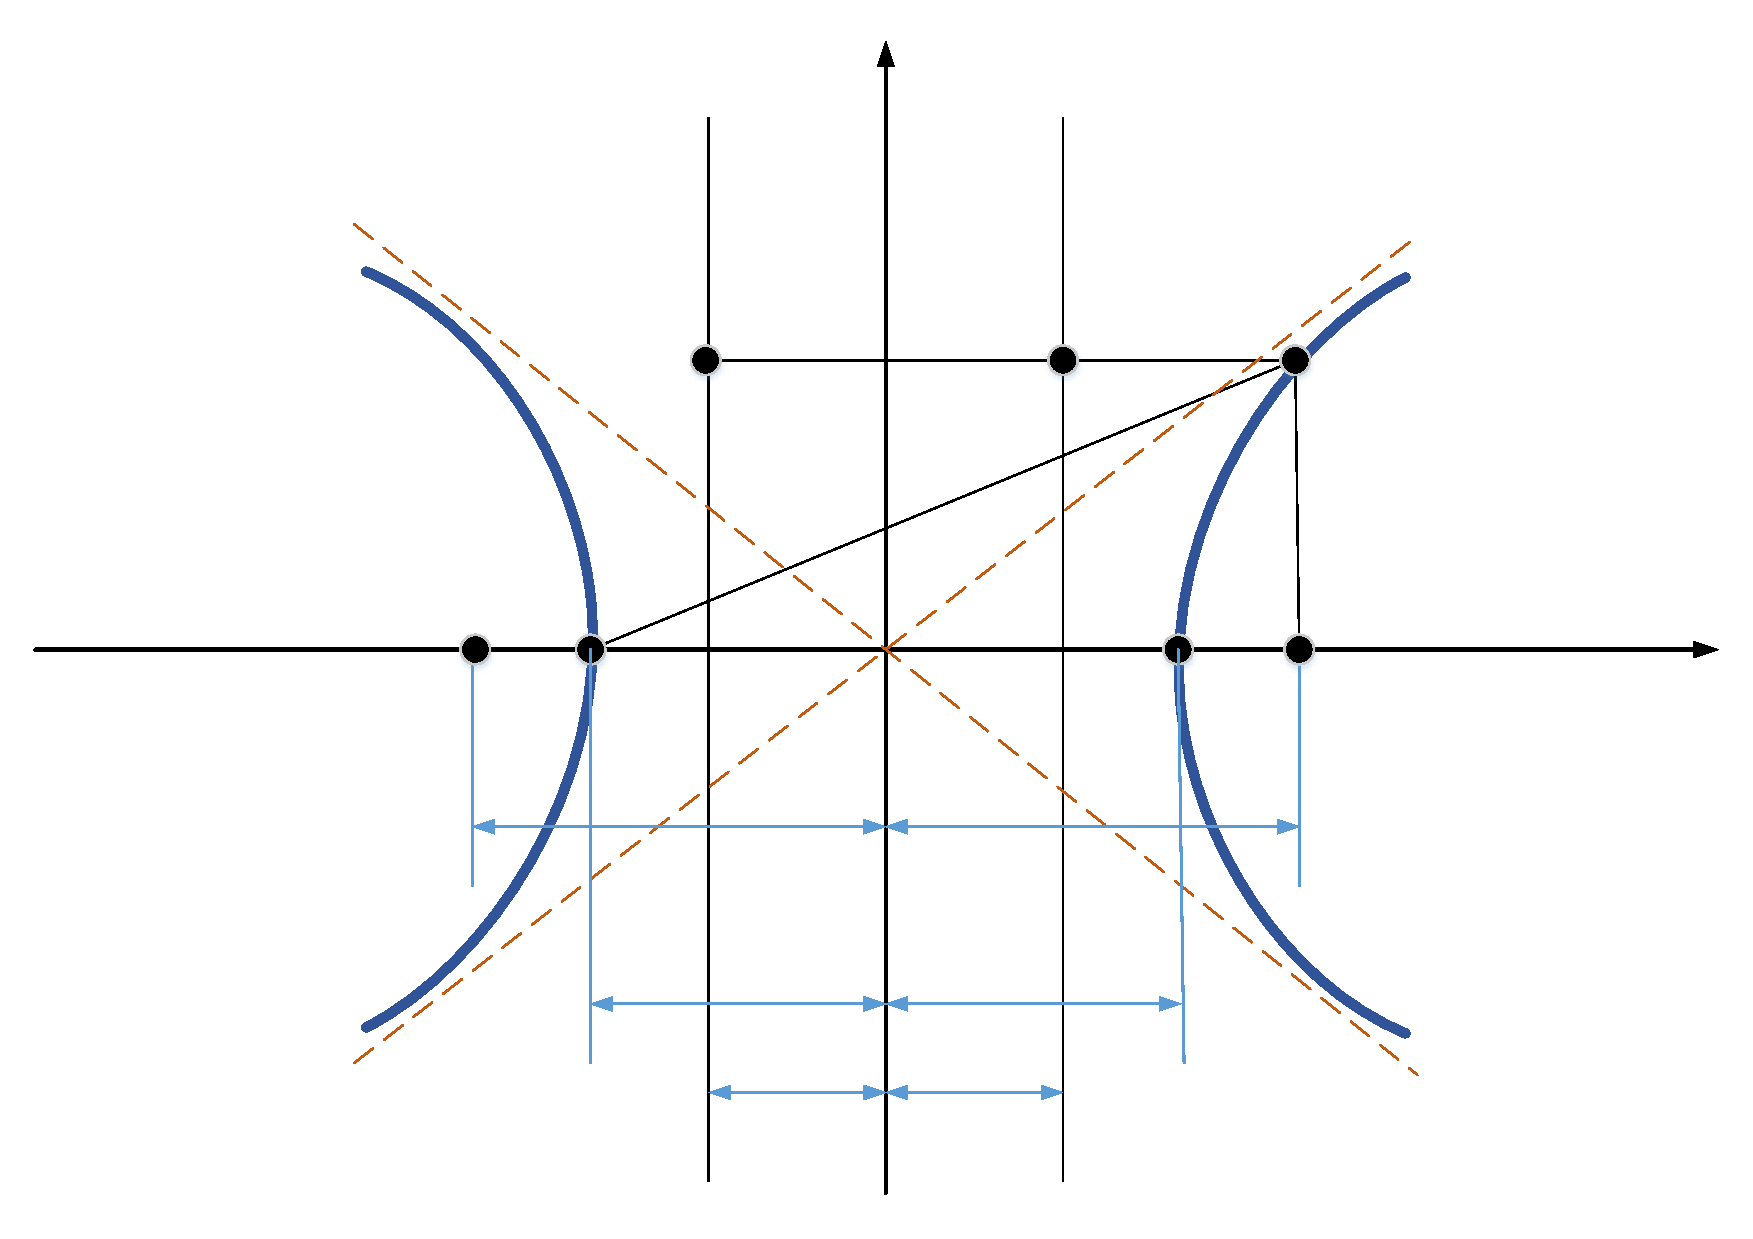
\includegraphics[width=0.55\textwidth]{Drawing5_1.pdf}
\caption{Graph and features of the hyperbola $\dfrac{x_T^2}{\alpha^2 x_A^2} - \dfrac{y_T^2}{(1-\alpha^2)x_A^2}=1$ }
\label{hyperbola graph}
\end{figure}


In passing, we note that though equation (\ref{hyperbola}) was obtained herein as the special case $(\gamma=1)$ of equation $(\ref{poly2})$, we have first obtained it by a rephrasing of the criticality condition (\ref{case3_SD}) which holds for $\gamma=1$.\\


Now we note that the left branch of the hyperbola lies entirely in $R_{r}$ and hence it is rejected. The right branch of the hyperbola is the required Voronoi diagram, and it is bordering the escape region $R_{e}$ which extends to its left. Clearly, it is an enlargement of the reachability region $R_{r}$. Likewise, we expect the escape region to be a subset of the $AD$ Apollonius circle in Fig. \ref{2_g<1} where $\gamma<1$, and to be a superset of this circle in Fig. \ref{2_g>1} where $\gamma>1$.   

Figure \ref{gamma=1} is a sketch of the hyperbola (\ref{hyperbola}) for $\alpha=0.25$. the figure stresses that the right branch of the hyperbola is accepted as a Voronoi diagram while the left branch is rejected as such. Figure 5.3 is computer generated Voronoi diagrams for $\gamma=1$ and $\alpha$ varying from 0 (the $y_T$-axis) to slightly less than 1 (the straight-line ray emanating from $\boldsymbol{A}$ and coinciding with the $x_T$-axis).

Now, we come to a novel and really important contribution of this paper, where we visualize the escape regions in the case of a fast Defender and a slow Defender. Figure \ref{gamma=0.8} shows the $AD$-Apollonius circle for $\gamma=0.8$ and $x_A=4$ for which $\boldsymbol{I_1}=(0.444,0)$, $\boldsymbol{E_1}=(36,0)$, $\boldsymbol{O_1}=(18.22,0)$, and $r_1=17.78$. Imposed on this circle is the quartic curve given by (\ref{poly2}) which consists of two closed curves. There is one closed curve entirely outside the $AD$-Apollonius circle, i.e., entirely inside the Reachability region $R_r$ and hence is rejected. The other closed curve is entirely inside the $AD$-Apollonius circle, i.e., the reachability region $R_r$ and hence it is accepted as the Voronoi diagram. The escape region (safe region) is the \textit{unshaded} area in this figure. Figure 5.5 generalizes Fig. \ref{gamma=0.8} by demonstrating various accepted branches of the Voronoi diagram for $\gamma=0.8$ and $\alpha$ as s parameter ranging from 0 (the $AD$-Apollonius circle) to a value approaching 1 from below (a closed curve collapsing to one barely encircling point A). This means that as $\alpha$ increases from 0 to 1, the safe or escape region expands from the exterior of the $AD$-Apollonius circle to almost the whole $x_T-y_T$ plane (excluding point A).


Now, we discuss the strikingly similar or dual case of a slow Defender. Figure \ref{gamma=1.25} shows the $AD$-Apollonius circle for $\gamma=1.25$ and $x_A=4$ for which $\boldsymbol{I_1}=(-0.444,0)$, $\boldsymbol{E_1}=(-36,0)$, $\boldsymbol{O_1}=(-18.22,0)$, $r_1=17.78$. Imposed on this circle is the quartic curve given by (\ref{poly2}). Note that the whole graph in Fig. \ref{gamma=1.25} is a \textit{mirror image} of that in Fig. \ref{gamma=0.8}. The quartic curve again consists of two closed curves. There is one closed curve entirely inside the $AD$-Apollonius circle. i.e., entirely inside the Reachability region $R_r$ and hence is rejected. The other closed curve is entirely outside the $AD$-Apollonius circle, i.e., entirely outside the Reachability region $R_r$, and hence is accepted as the Voronoi diagram. The escape region (safe region) is the \textit{shaded} area in this figure. Figure 5.7 generalizes Fig. \ref{gamma=1.25} by demonstrating various accepted branches of the Voronoi diagram for $\gamma=1.25$ and $\alpha$ as a parameter ranging from 0 (the $AD$-Apollonius circle) to a value approaching 1 from below.\\ 
    

In passing, we discuss the situation of $\gamma=0$ (when the Target does not move at all). In this case the $TA$ circle collapse into a single point $\boldsymbol{T}$ and the critically condition (\ref{generaleq4}) reduces to 

\begin{equation}
(1-\alpha^{2})d^{2}= 4 \gamma^{2} x_{T} x_{A}
\end{equation}

which can readily be written as 
\begin{equation}
(x_T-(\dfrac{1+\gamma^2}{1-\gamma^2})x_A)^2+(y_T-0)^2
=(\dfrac{2\gamma x_{A}}{1-\gamma^{2}})^{2}
\end{equation}

an equation that can be identified as the equation of the $AD$ Apollonius circle in the $Y_T-X_T$ coordinates.
This circle serves as the Voronoi diagram for $\alpha=0$, a fact confirming our assertion that the escape region $R_e$ reduces to the reachability region $R_r$ when $\alpha=0$. Likewise, when $\gamma=1$, imposing the condition $\alpha=0$ on the condition (\ref{case3_SD}) results in 
\begin{equation}
x_T=0
\end{equation} 
which means that the right branch of the hyperbolic Voronoi diagram (\ref{hyperbola}) degenerates into the $y_T-$axis (the perpendicular bisector of $\overline{AD}$) and again the region $R_e$ concides with the region $R_r$ in this case.


\begin{figure}[htb]
\centering
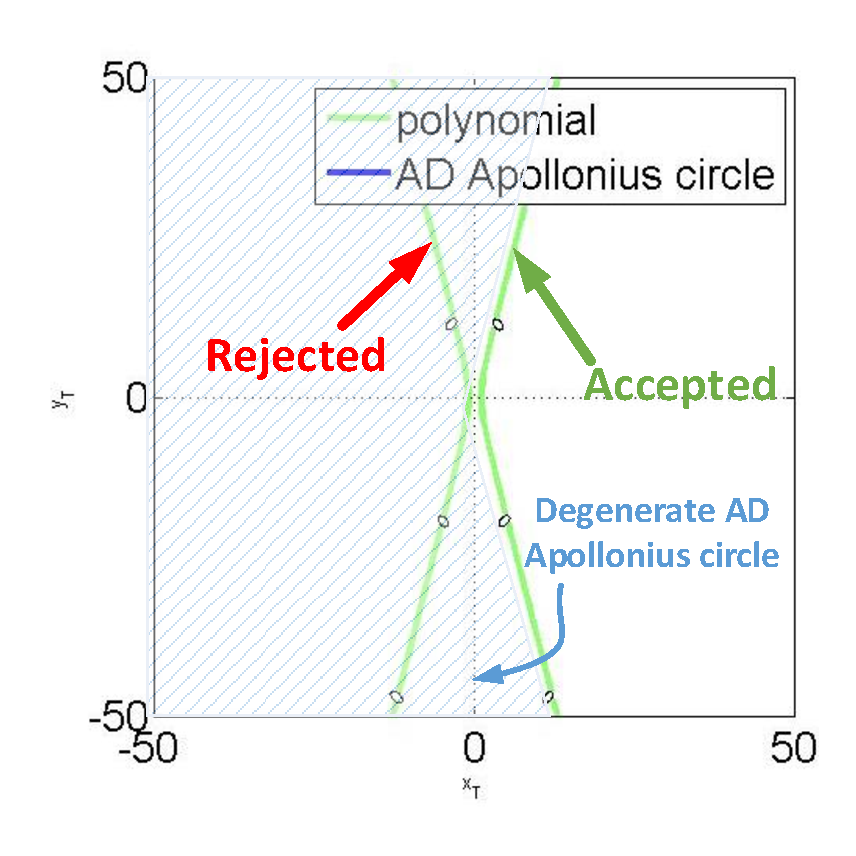
\includegraphics[width=0.75\columnwidth]{g_1.pdf}
\caption{Generated computer output for the Voronoi diagram bordering the safe region for $x_A=4,\ \alpha=0.25,\ \gamma=1$ (the safe region is the shaded area)}
\label{gamma=1}
\end{figure}

\begin{figure}[htb]
\centering
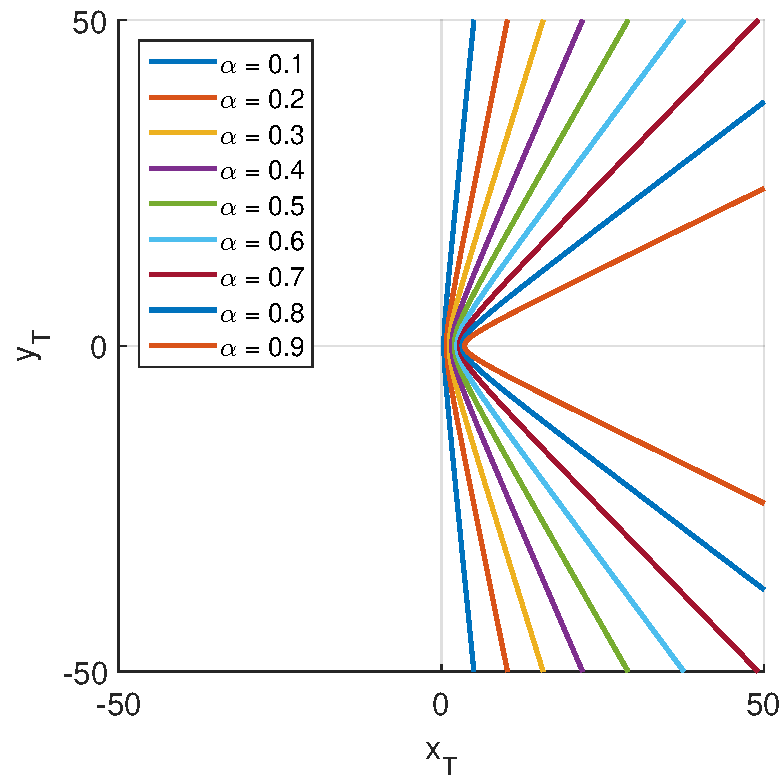
\includegraphics[width=0.75\columnwidth]{VAR_alpha_g_1.pdf}
\caption{Various accepted branches of the voronoi diagram for $\gamma=1$ and $\alpha$ as a parameter ranging from 0 to 1. These curves are computer generated from (\ref{poly2}) and (\ref{hyperbola})}
\label{VAR_alpha_gamma=1}
\end{figure}


\begin{figure}[htb]
\centering
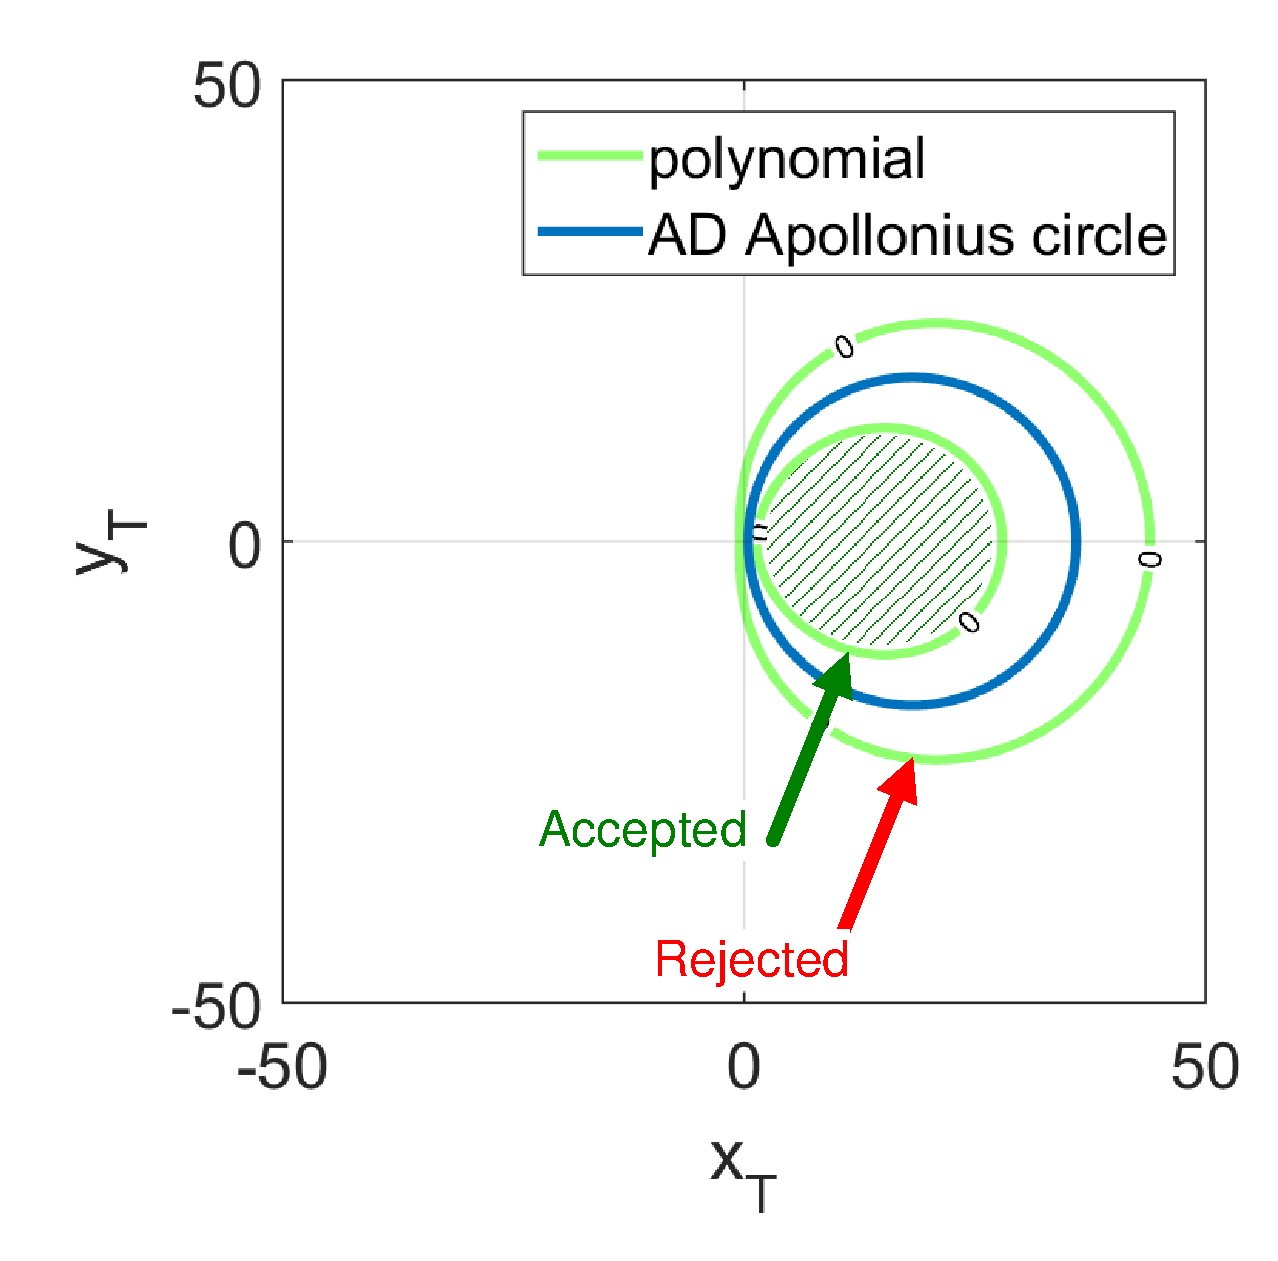
\includegraphics[width=0.75\columnwidth]{marked_circle_curve_g_0p8.pdf}
\caption{generated computer output for the Voronoi diagram bordering the safe region for $x_A=4,\ \alpha=0.25,\ \gamma=0.8$ (the safe region is the unshaded area) the quartic in (\ref{poly1}) or (\ref{poly2}) produces two closed curves: one outside the $AD$-Apollonius circle (rejected) and the other inside the circle (accepted as the Voronoi diagram)}
\label{gamma=0.8}
\end{figure}


\begin{figure}[htb]
\centering
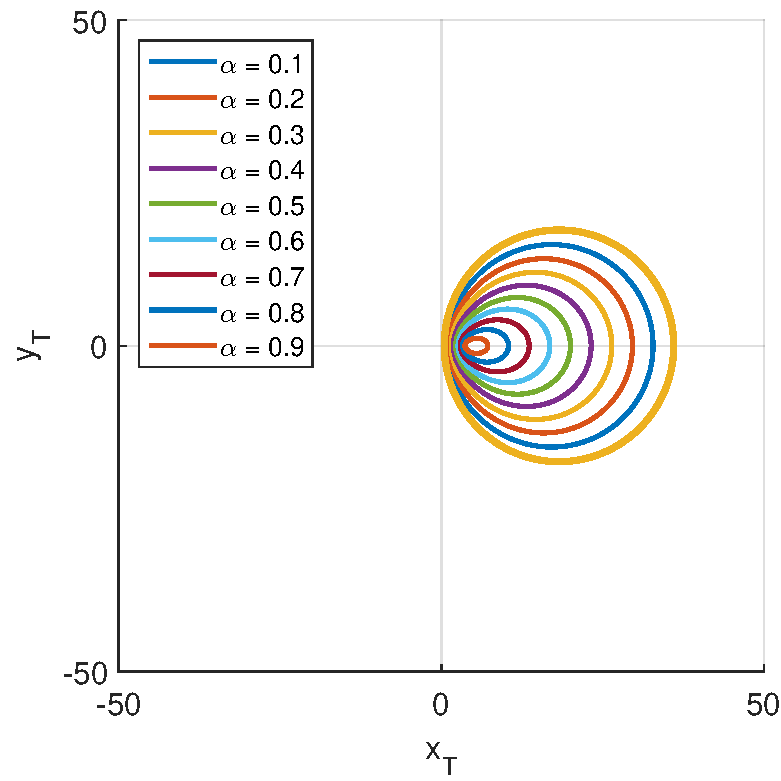
\includegraphics[width=0.75\columnwidth]{VAR_alpha_g_0p8.pdf}
\caption{Various accepted branches of the voronoi diagram for $\gamma=0.8$ and $\alpha$ as a parameter ranging from 0 to 1. These curves are computer generated from (\ref{poly2}) and (\ref{hyperbola})}
\label{VAR_alpha_gamma=0.8}
\end{figure}


\begin{figure}[htb]
\centering
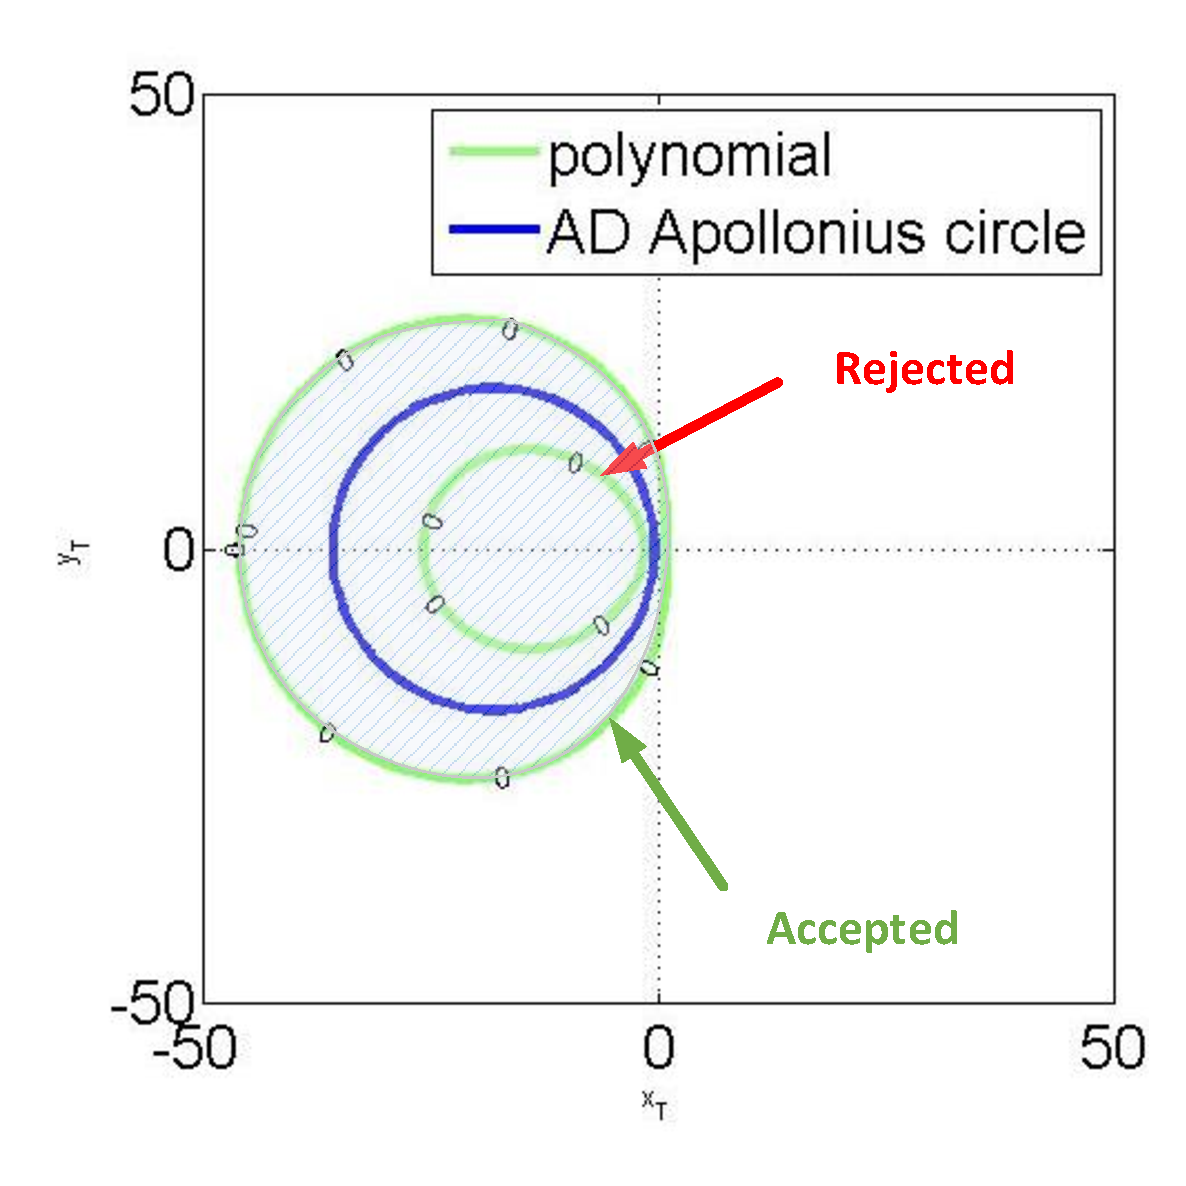
\includegraphics[width=0.75\columnwidth]{g_1p25.pdf}
\caption{generated computer output for the Voronoi diagram bordering the safe region for $x_A=4,\ \alpha=0.25,\ \gamma=1.25$ (the safe region is the shaded area) the quartic in (\ref{poly1}) or (\ref{poly2}) produces two closed curves: one inside the $AD$-Apollonius circle (rejected) and the other outside the circle (accepted as the Voronoi diagram)}
\label{gamma=1.25}
\end{figure}

\begin{figure}[htb]
\centering
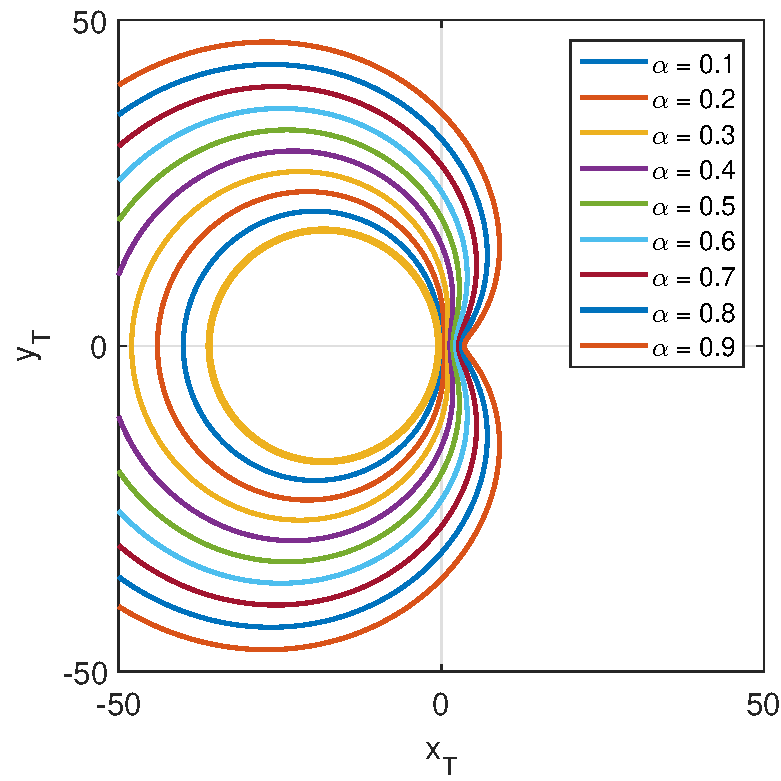
\includegraphics[width=0.75\columnwidth]{VAR_alpha_g_1p25.pdf}
\caption{Various accepted branches of the voronoi diagram for $\gamma=1.25$ and $\alpha$ as a parameter ranging from 0 to 1. These curves are computer generated from (\ref{poly2}) and (\ref{hyperbola})}
\label{VAR_alpha_gamma=1.25}
\end{figure}

% =========================================
\section{CONCLUSION AND FUTURE WORK}
This paper offered a unified analytic solution of the $TAD$ problem in which an Attacker is pursuing a Target while attempting to evade a Defender. The paper reviews and extends the work that has recently appeared in \cite{pachter2014active,garcia2015active,garcia2015escape}, beside making the following new contributions:

\begin{enumerate}
\item The paper covers all cases for the ratio $\gamma$ of the Attacker's speed w.r.t. the Defender's speed. It treats the case of a slow Defender ($\gamma>1$) for the first time, and presents this case along with the case of a fast Defender ($\gamma<1$) discussed in \cite{garcia2015active} and the case of a similar Defender ($\gamma=1$), discussed earlier in \cite{pachter2014active,garcia2015escape}.
\item The paper demonstrates a striking increase in complexity when $\gamma\neq1$ compared with the case $\gamma=1$. It also demonstrates some sort of \textit{duality} between the two cases of ($\gamma<1$) and ($\gamma>1$).
\item The paper develops novel analytic expressions for the Voronoi diagrams bordering the escape regions when ($\gamma<1$) or ($\gamma>1$). These expressions are more complex than the ones obtained in [3] for ($\gamma=1$), and reduce to it as a limiting case.
\item The paper offers a tutorial exposition of the $TAD$ problem, uses simple arguments of plane geometry to develop the necessary Apollonius circles, utilizes equalities rather than inequalities in developing Voronoi diagrams, and pays careful attention to the inadvertent inclusion of extraneous solutions so as to justify their subsequent rejection.
\item The paper supplements its analysis with extensive computations for the critical speed ratio Voronoi diagrams. The results obtained encompass all possible values of $\gamma$, and they reduce to the already available results for $\gamma=1$.
\end{enumerate}  

Some possible extensions of the current work that warrant further exploration include:
\begin{enumerate}
\item Further analysis of the quartic equation obtained for the Voronoi diagram when $\gamma\neq1$, with an aim to \textit{split} it into two factors representing the rejected and accepted branches of the diagram.
\item Investigation of the sixth-degree complex polynomial equation for the optimal interception angle to get some \textit{insight} about its six roots, and to find a better way for \textit{selecting} the desirable root.
\item Relaxation of some of the assumptions used in this study. In particular, it is very interesting to consider the possibility of \textit{variable} rather than constant speeds for the three agents.
\item Addition of an element of \textit{uncertainty} to the computation. For example, we might assume that the initial positions of the three agents are not deterministic but \textit{stochastic} or \textit{fuzzy}.
\item Extension of the current work to a more general situation involving several Targets, several Attackers and/or several Defenders.     
\end{enumerate} 

% =========================================
% =========================================
% =========================================

%\section*{Acknowledgment}
%
%The authors would like to thank Prof. Ali Rushdi and Dr. Ahmad Rushdi.

% =========================================
%\bibliographystyle{myieeetr}
%\bibliography{references} 
%% ===================================================
%% The Appendices part is started with the command \appendix;
%% appendix sections are then done as normal sections
\appendix

%% \section{}
%% \label{}

%% If you have bibdatabase file and want bibtex to generate the
%% bibitems, please use
%%
\section*{References}
\bibliographystyle{elsarticle-num} 
\bibliography{references}

%% else use the following coding to input the bibitems directly in the
%% TeX file.

%\begin{thebibliography}{00}
%%% \bibitem{label}
%%% Text of bibliographic item
%\bibitem{}
%\end{thebibliography}
\end{document}
\endinput
%% ===================================================